
\chapter{Enterprise Response Tooling}
\newpage

\section{Velociraptor}
Use Velociraptor to collect evidence, hunt for IOCs or just to monitor for something to happen. For that purpose, there are different kinds of client and server artifacts (scripts to collect stuff) some general and some that trigger on events which you could use for monitoring.

Usually, connected clients stats curve reflects very much the general working hours

Here's a LaTeX template for documenting Velociraptor:

Velociraptor is an endpoint visibility and monitoring tool designed for digital forensics and incident response (DFIR).

\subsection{Core Capabilities}
\subsubsection{Endpoint Monitoring}
\begin{itemize}
    \item Real-time system monitoring
    \item Cross-platform support (Windows, Linux, macOS)
    \item VQL (Velociraptor Query Language) implementation
\end{itemize}

\subsection{Technical Features}
\begin{itemize}
    \item Memory analysis \& acquisition
    \item File system monitoring
    \item Process execution tracking
    \item Network connection monitoring
    \item Registry analysis (Windows)
\end{itemize}

\subsection{Architecture}
\subsubsection{Client-Server Model}
\begin{verbatim}
Client --> [Encrypted Channel] --> Server
\end{verbatim}

\section{Use Cases}
\begin{enumerate}
    \item Incident Response
    \item Threat Hunting
    \item Compliance Monitoring
    \item Digital Forensics
\end{enumerate}

\section{VQL Example}
\begin{lstlisting}[language=SQL]
SELECT * FROM processes 
WHERE name =~ "suspicious_process"
\end{lstlisting}


\subsection{User Interface Basics}

\subsubsection*{Search Connected Clients}
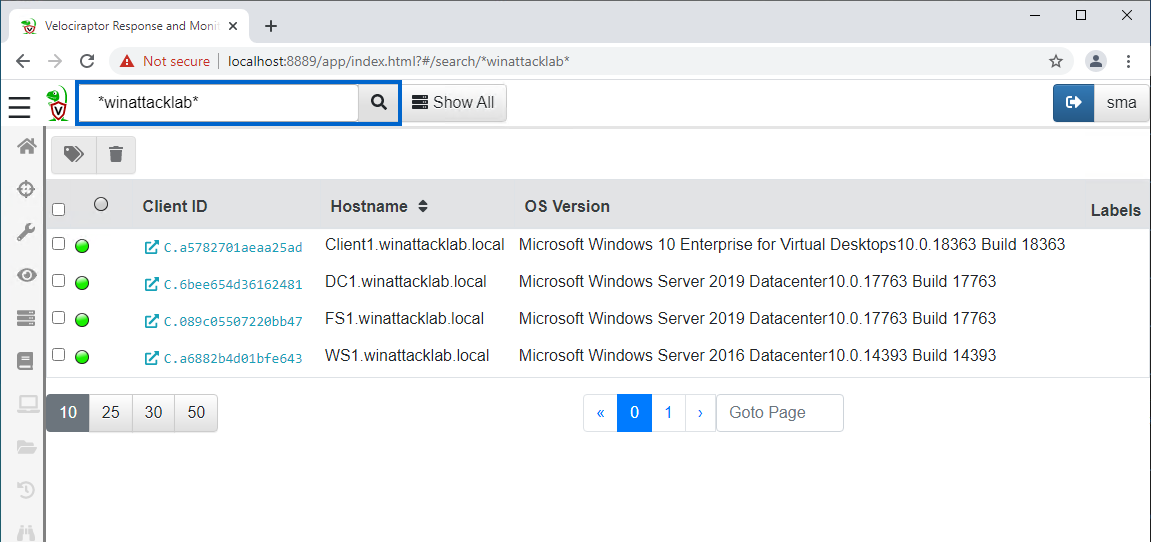
\includegraphics[width=\textwidth]{resources/06-velociraptor-interface-01.png}

\subsubsection*{Access Connected Client}
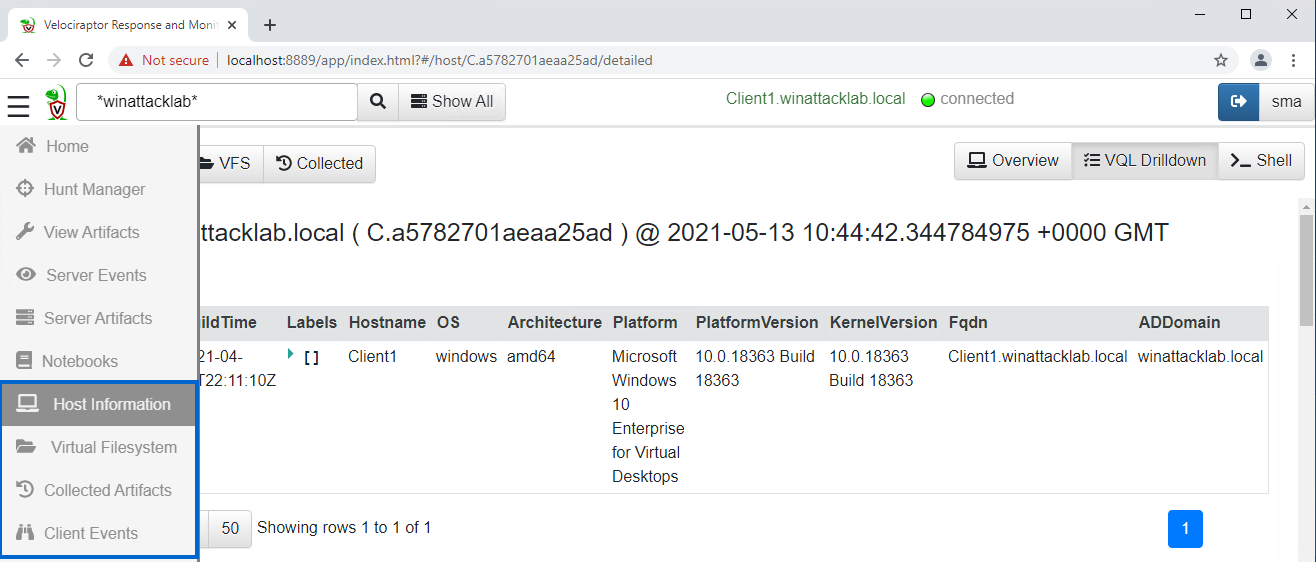
\includegraphics[width=\textwidth]{resources/06-velociraptor-interface-02.png}

\subsubsection*{Virtual File System}
\begin{itemize}
  \item \textbf{File}: File system access based on OS FS API
  \item \textbf{NTFS}: NTFS raw parsing filesystem access
  \item \textbf{Registry}: Windows Registry access using the Registry API
  \item \textbf{Artifacts}: Artifacts collected from the client incl. type and time in Velociraptor Artifacts are commands and scripts that actually grab some data (we usually call these artifacts) from clients.
\end{itemize}
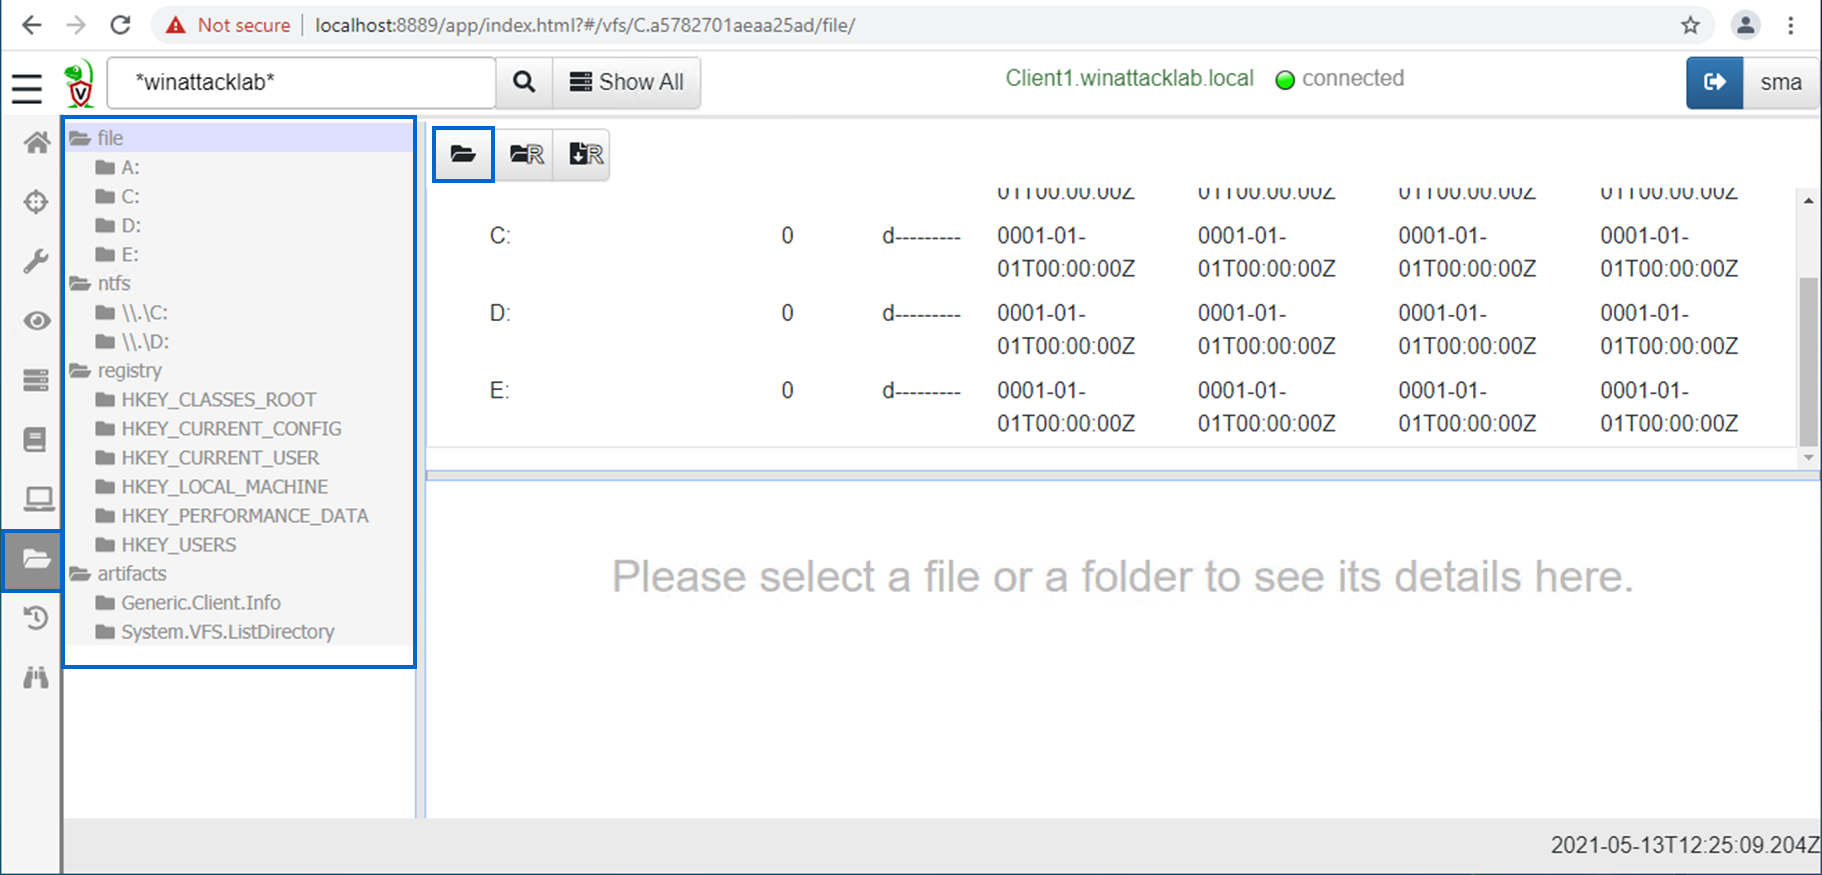
\includegraphics[width=\textwidth]{resources/06-velociraptor-interface-03.png}

\subsubsection*{File Download (collection)}
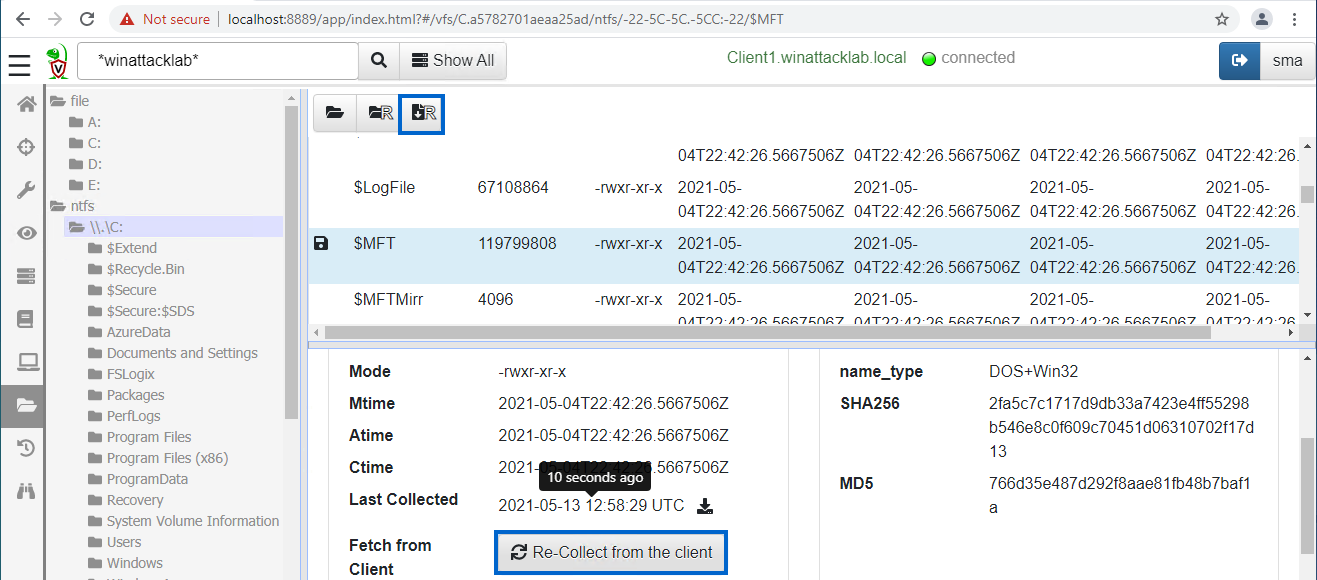
\includegraphics[width=\textwidth]{resources/06-velociraptor-interface-04.png}

You may collect files individually (lower button) or an entire folder recursively (top button). Files get marked with the floppy once available on the server.

\subsubsection*{Velociraptor VFS}
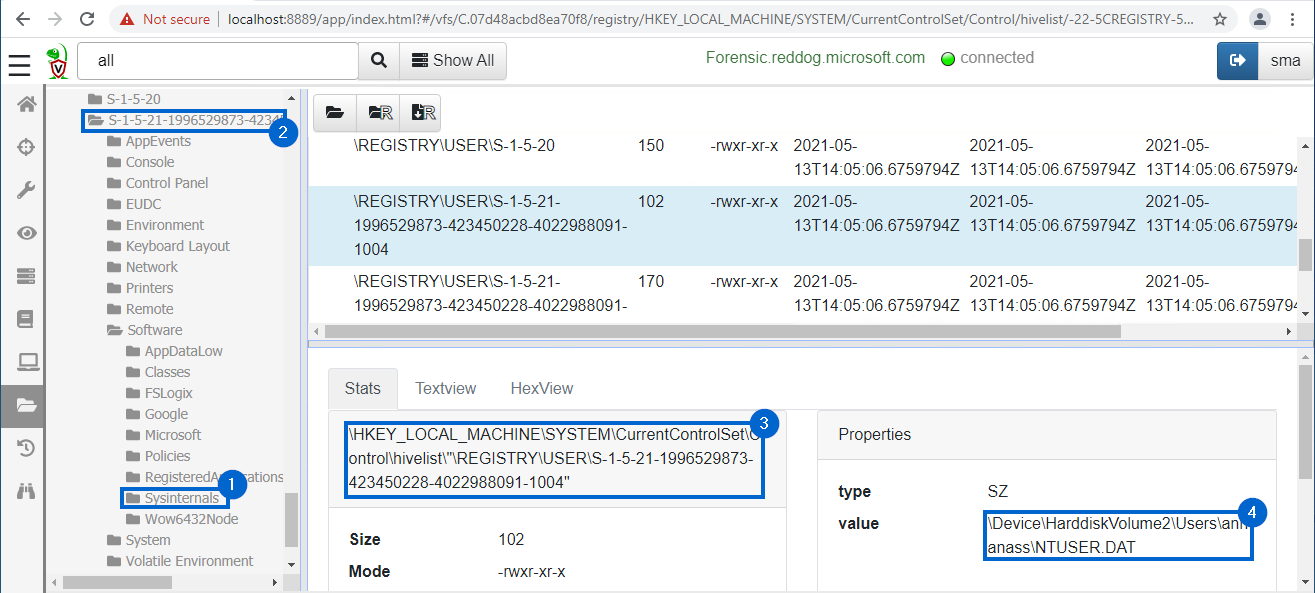
\includegraphics[width=\textwidth]{resources/06-velociraptor-interface-05.png}

\subsection{Velociraptor Artifacts}

Velociraptor is a query language engine. Basically everything is a query (VQL).
Artifacts aim to encapsulate evidence collection

\begin{itemize}
  \item Structure is YAML
  \item Ideally includes comments
  \item Allow for customization where reasonable
  \item Recursion. Use Artifacts in the query language
\end{itemize}

\subsection{Velociratpro Hunts}
Hunting enables you to collect the same artifacts over an entire fleet.
\begin{itemize}
  \item Only systems that are connected will participate in the hunt
  \item Only systems that are connected will deliver results
  \item Hunts are run for quite some time (days), repeatedly
  \item Hunts may be restricted by label or OS
\end{itemize}

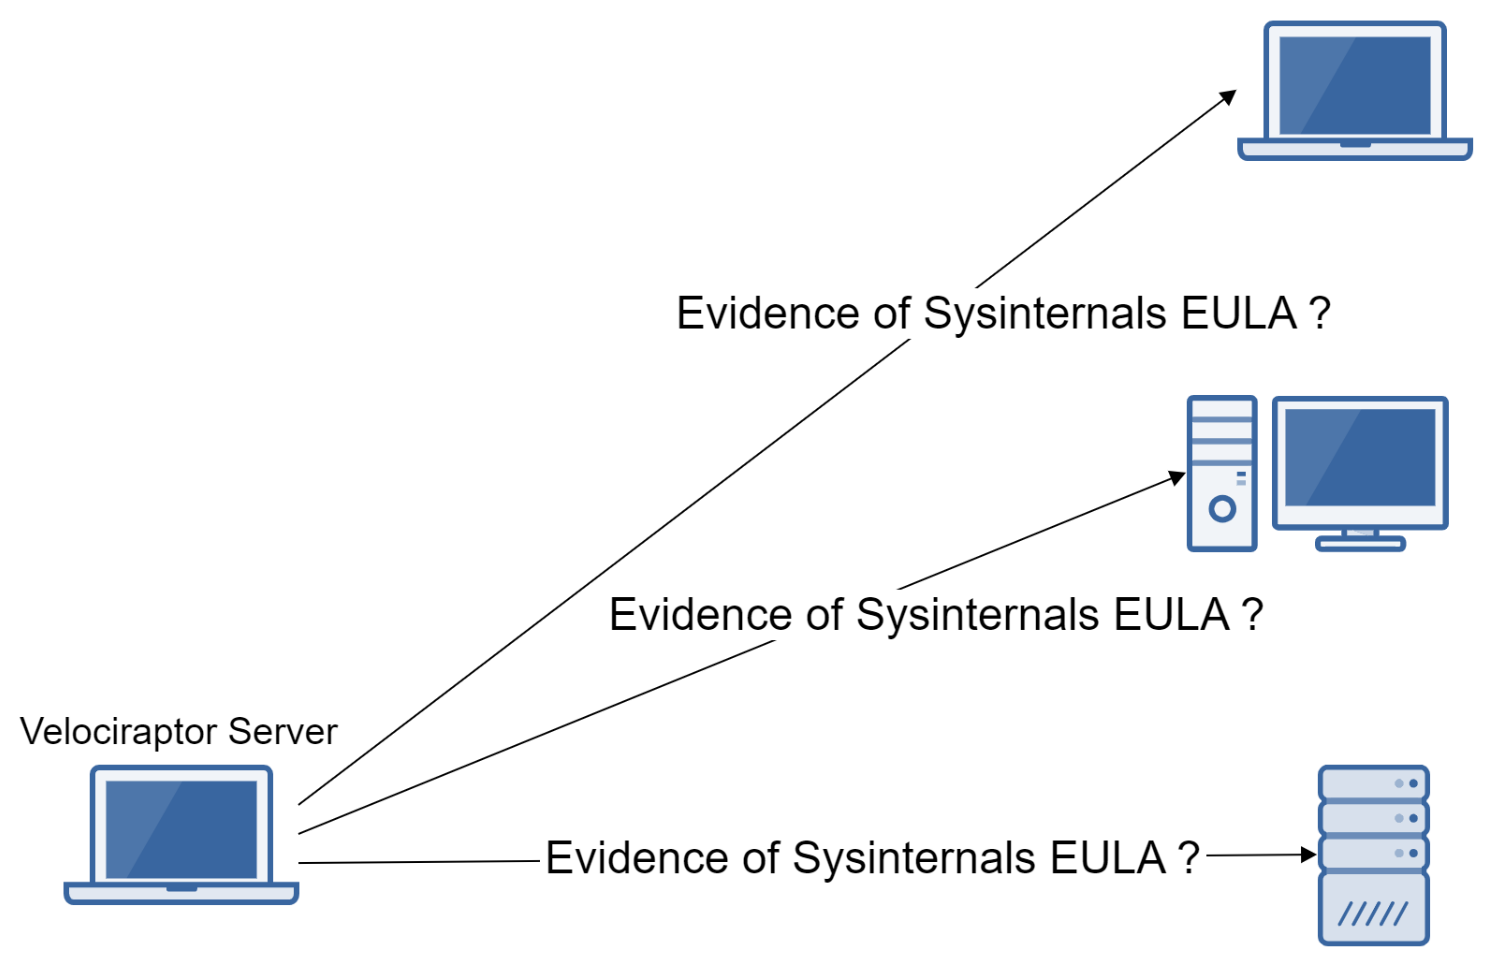
\includegraphics[width=\textwidth]{resources/06-velociraptor-hunt.png}

\subsubsection*{Hunt Example}
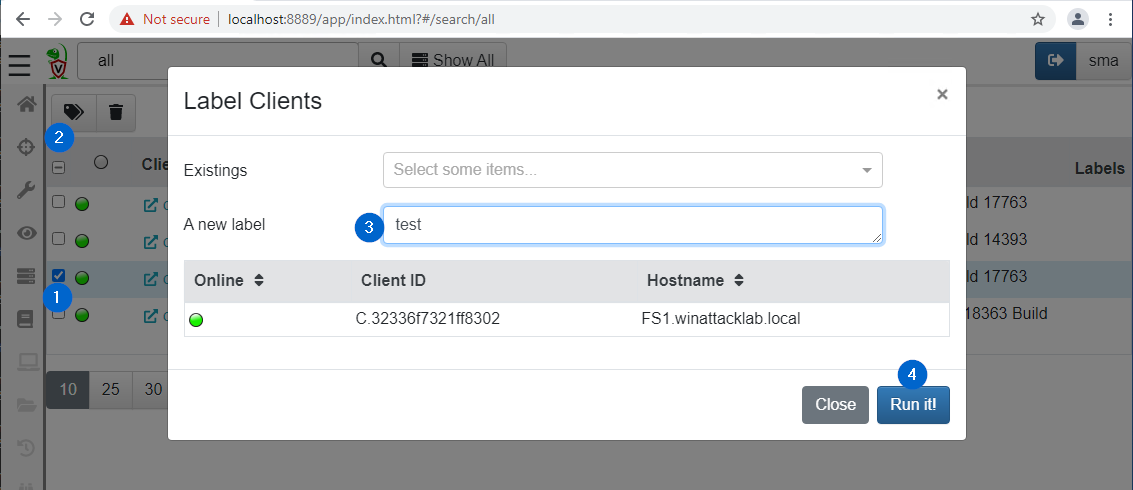
\includegraphics[width=\textwidth]{resources/06-velociraptor-hunt-2.png}
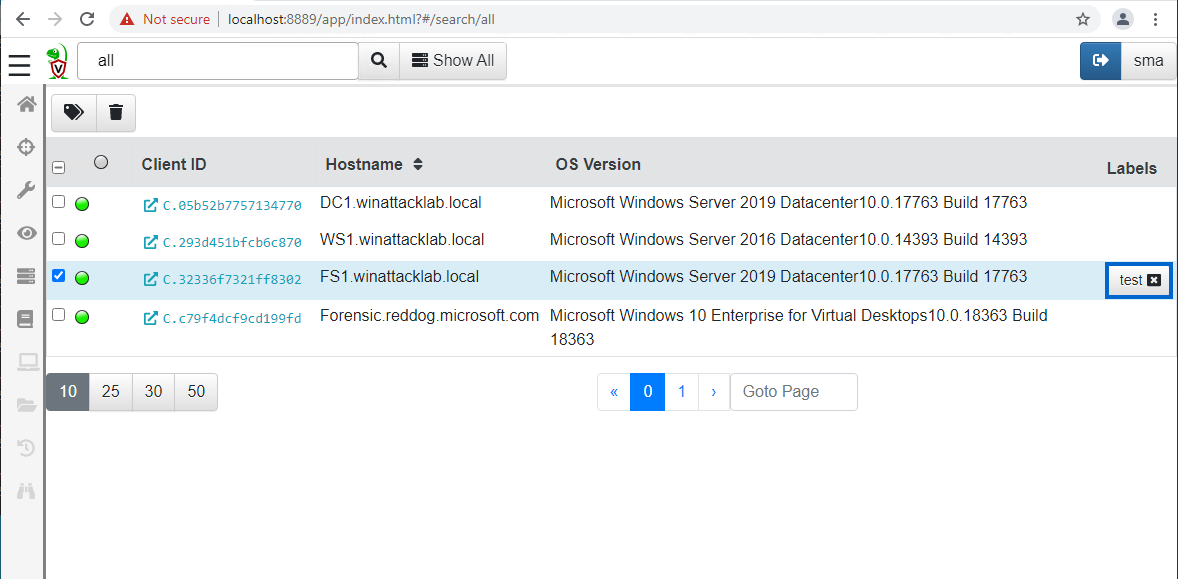
\includegraphics[width=\textwidth]{resources/06-velociraptor-hunt-3.png}
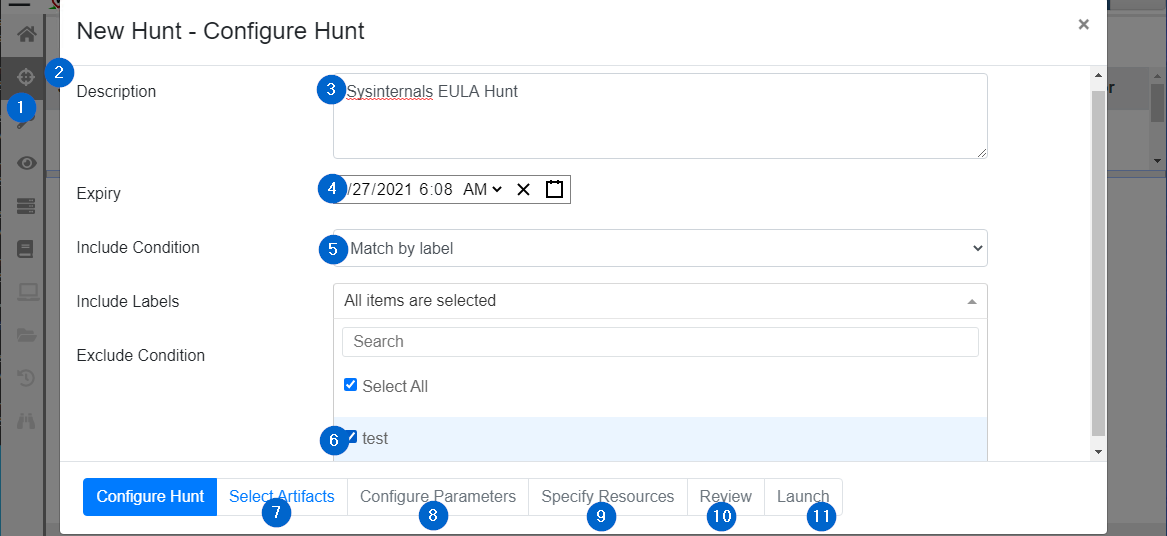
\includegraphics[width=\textwidth]{resources/06-velociraptor-hunt-4.png}
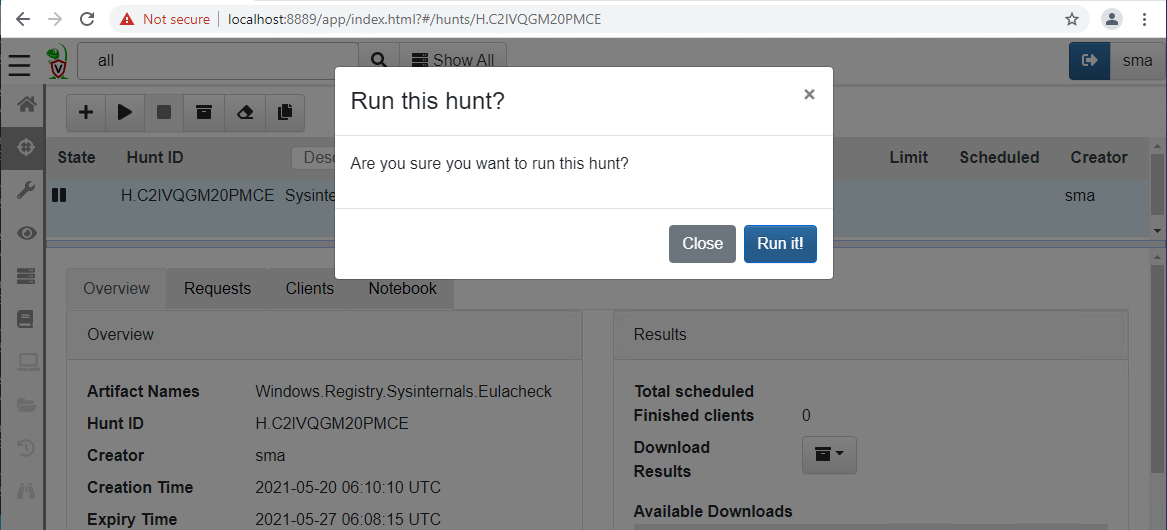
\includegraphics[width=\textwidth]{resources/06-velociraptor-hunt-5.png}

\subsection{Active Containment}
Active containment enables real-time incident response through Velociraptor's endpoint control capabilities.

\subsubsection*{Core Functions}
\begin{itemize}
    \item Process termination
    \item Network isolation
    \item System quarantine
    \item Account deactivation
    \item Persistence removal
    \item Execution blocking
\end{itemize}

\subsubsection*{VQL Implementation Examples}
\begin{lstlisting}[language=SQL]
# Kill malicious process
SELECT kill(pid=ProcessPID) 
FROM processes 
WHERE name=MaliciousProcess

# Block suspicious connections
SELECT block_ip(ip=SuspiciousIP) 
FROM netstat 
WHERE state="ESTABLISHED"
\end{lstlisting}

\subsubsection*{Key Features}
\begin{itemize}
    \item Remote execution capability
    \item Customizable response workflows
    \item Trigger-based automation
    \item Comprehensive audit logging
    \item Reversible containment actions
    \item Role-based access control
\end{itemize}

Active containment facilitates rapid incident response while preserving forensic evidence for investigation and analysis.


\subsection{Collecting Files}
Incident Response may require for quick conservation of a number artifacts to be analyzed later on or being given somewhere else for analysis. With Velociraptor comes the KapeFiles Client Artifact which is a great collector of relevant files.

Approaches
\begin{itemize}
  \item Run hunt or collection within the Velociraptor Infrastructure
  \item Run standalone collector with Velociraptor
\end{itemize}

What to collect
\begin{itemize}
  \item \_BasicCollection
  \item \_SANS\_Triage
  \item \_KapeTriage
\end{itemize}

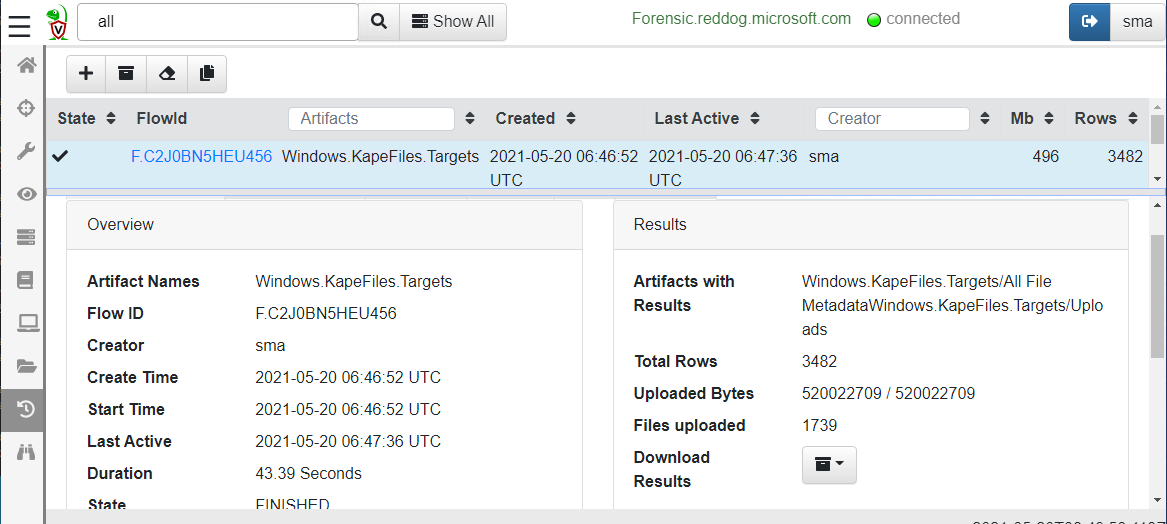
\includegraphics[width=\textwidth]{resources/06-collecting-files.png}
Collection Stats from the Forensics Client
\begin{itemize}
  \item Collection ran for 45 seconds
  \item Collection returned 1750 files
  \item 1750 files sum up to 500MB (most for the MFT, NTFS Journals, System registry)
  \item 1750 files zipped for download 70MB
  \item The top level includes the hunt configuration details including some meta info.
  \item The client folder contain the results per client workstation name.
  \item Within the collections flow folder. The uploaded files are separated by the accessor they got collected with.
  \item Thus \$MFT et al will be available from the ntfs folder. Any common files from the auto folder.
  \item Kape does by default create a VHDX and timestomp files in it. So non-tech savvy folks may browse it like a real disk. You are better of by using the \$MFT directly.
\end{itemize}

Note, the Forensics Client is a “pretty empty” system.

Collecting large files will not result in a memory bottleneck as Velociraptor throttles clients if needed. However, extensive hunts on machines or collection of user document folders, virtual machine images, memory dumps could easily jam your server its connection or fill your server its disk. Be careful!

\subsubsection*{Manual File Colection}

\begin{lstlisting}[basicstyle=\ttfamily]
# List Kape artifacts
Get-Command velociraptor.exe artifacts list '*Kape*'

# Show artifact details 
Get-Command velociraptor.exe artifacts show Windows.KapeFiles.Targets

# Collect artifacts
Get-Command velociraptor.exe artifacts collect Windows.KapeFiles.Targets --args_BasicCollection=Y --output=Collection_$env:computername.zip
\end{lstlisting}

\subsubsection*{Command Parameters}
\begin{itemize}
   \item \texttt{artifacts list} - Searches available artifacts
   \item \texttt{artifacts show} - Displays artifact details
   \item \texttt{artifacts collect} - Gathers specified artifacts
   \item \texttt{--args\_BasicCollection} - Sets collection parameters
   \item \texttt{--output} - Specifies output ZIP location
\end{itemize}

\subsubsection*{Metadata Storage}
Velociraptor stores the modified time in ZIP headers, with all timestamps available in:
\texttt{"Windows.KapeFiles.Targets/All File Metadata.json"}

\begin{lstlisting}[basicstyle=\ttfamily]
PS C:\> velociraptor.exe artifacts collect Windows.KapeFiles.Extract --argsContainerPath=Collection.zip --args OutputDirectory=/tmp
\end{lstlisting}

\subsubsection*{Timestamp Support}
\begin{itemize}
   \item Windows: Supports 3 timestamps (MAC time, excluding Btime)
   \item Linux: Supports 2 timestamps (Modified and Accessed)
\end{itemize}

Useful for tools requiring timestamp analysis (e.g., Prefetch analysis)

\begin{table}[h]
\begin{tabular}{|p{0.7\textwidth}|p{0.3\textwidth}|}
\hline
\textbf{Action, Artifact} & \textbf{Time} \\
\hline
Hunt for the full file path on a target systems using Windows.System.CmdShell with param "cmd.exe /c dir C:\\Users\\mpotter\\compass-test-file.txt" & Instant \\
\hline
Hunt for filename only using Windows.Forensics.FilenameSearch which searches the \$MFT & 30 sec \\
\hline
\lstinline|Creating a hash DB on target by Generic.Forensic.LocalHashes.Glob filtered for C:\\Users\\\*\*\\\* (4400 files)| & 4 min \\
\hline
Use Generic.Forensic.LocalHashes.Query to search a hash DB & Instant \\
\hline
Hunt for successful logons using Windows.EventLogs.ExplicitLogon on Client & 10 sec \\
\hline
Hunt for successful logons using Windows.EventLogs.ExplicitLogon on DC & 50 sec \\
\hline
Yara scan processes on a Windows box for a simple string & 5 min \\
\hline
Collecting 4GB of physical memory on a client => 1.2GB Zip Archive & 12 min \\
\hline
\end{tabular}
\caption{Velociraptor Speed to Numbers}
\end{table}

\subsection{Notebooks}

\begin{itemize}
  \item Create a New Notebook \\ 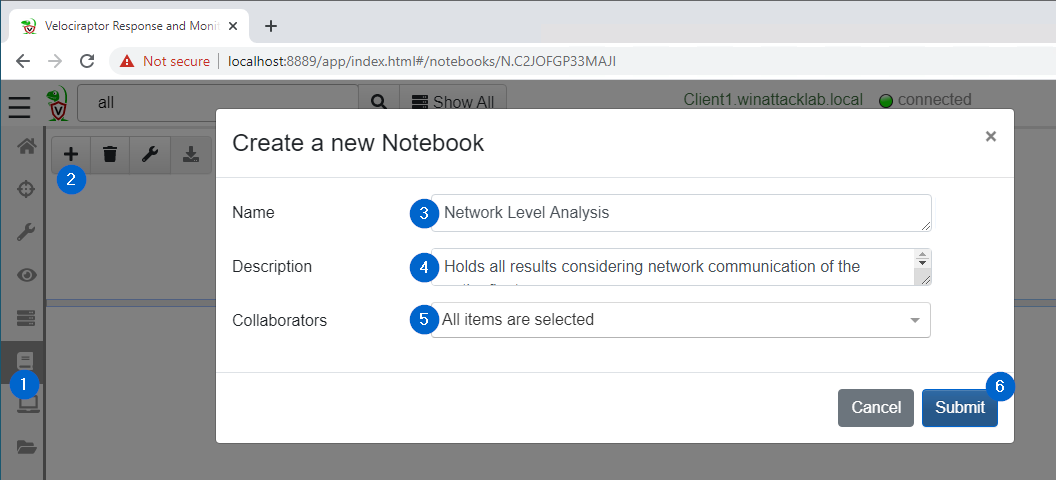
\includegraphics[width=\textwidth]{resources/06-velociraptor-notebooks-1.png}
  \item Edit Cells or Add New Cells using Existing Results (Hunts and Flows) \\ 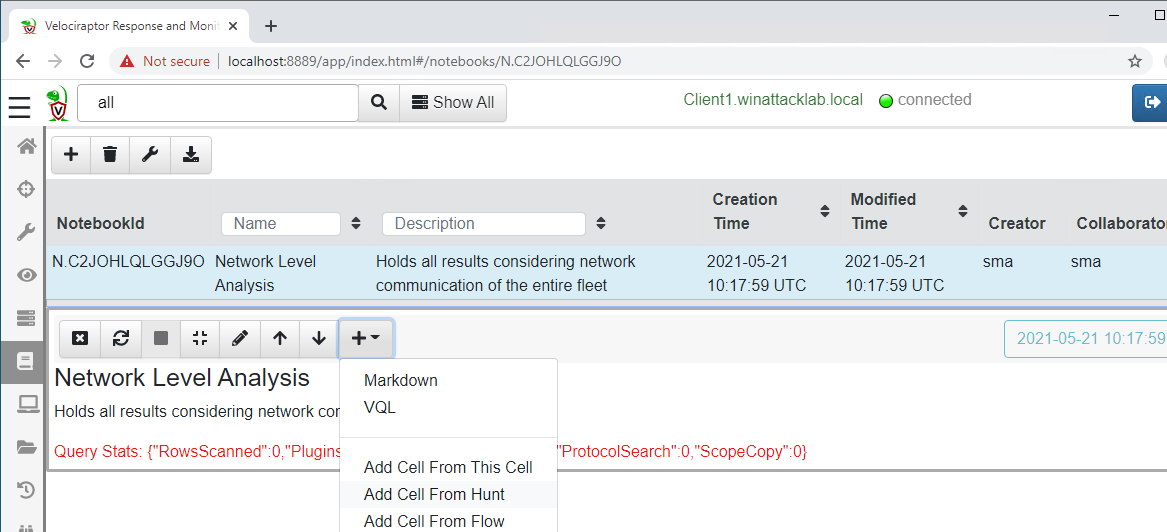
\includegraphics[width=\textwidth]{resources/06-velociraptor-notebooks-2.png}
  \item Add New VQL Query \\ 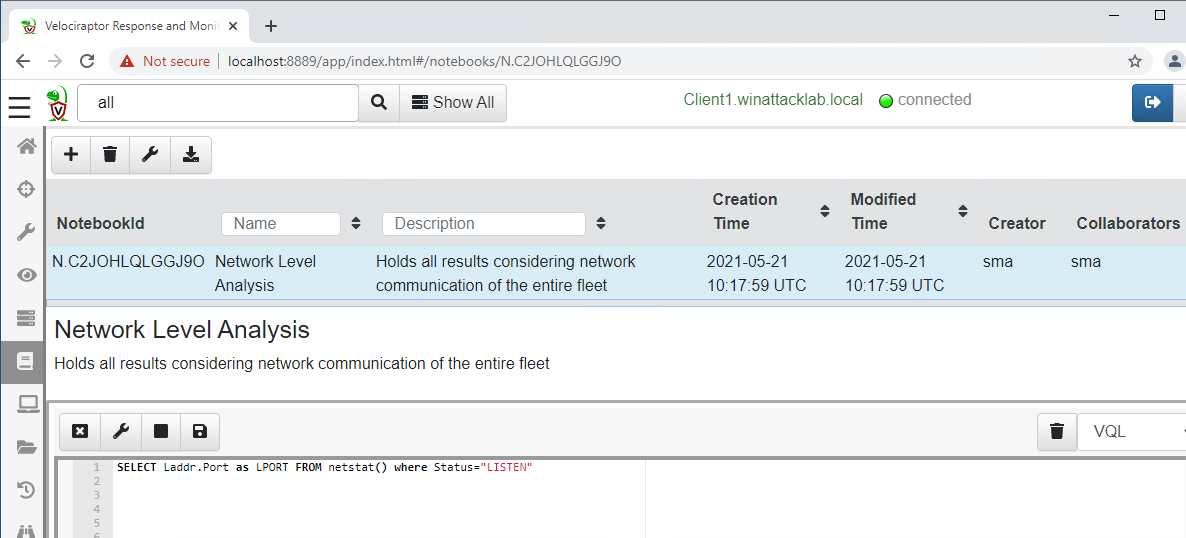
\includegraphics[width=\textwidth]{resources/06-velociraptor-notebooks-3.png}
  \item Results in Notebook Cells \\ 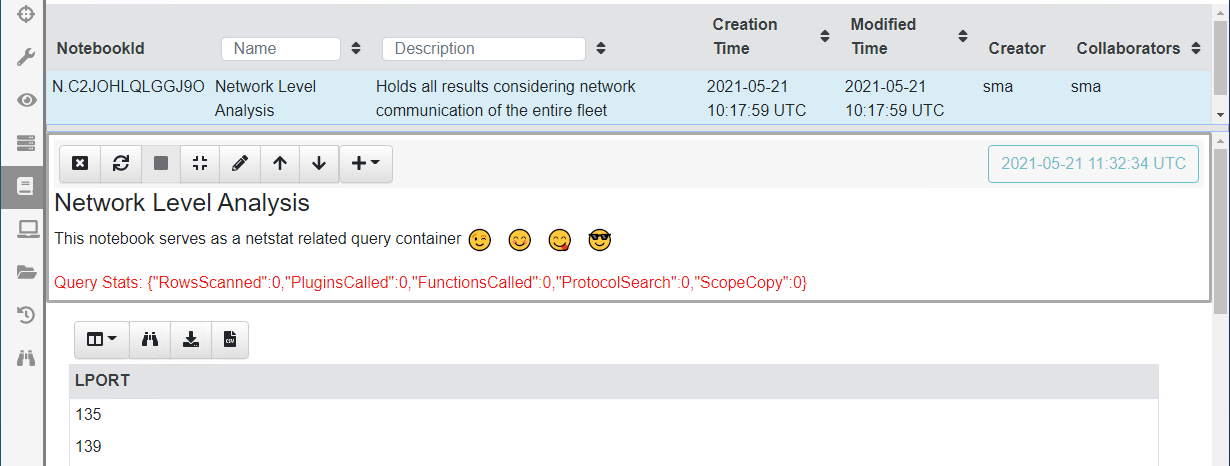
\includegraphics[width=\textwidth]{resources/06-velociraptor-notebooks-4.png}
  \item Tailor Flow Results (e.g. filter a Pslist Artifact output) \\ 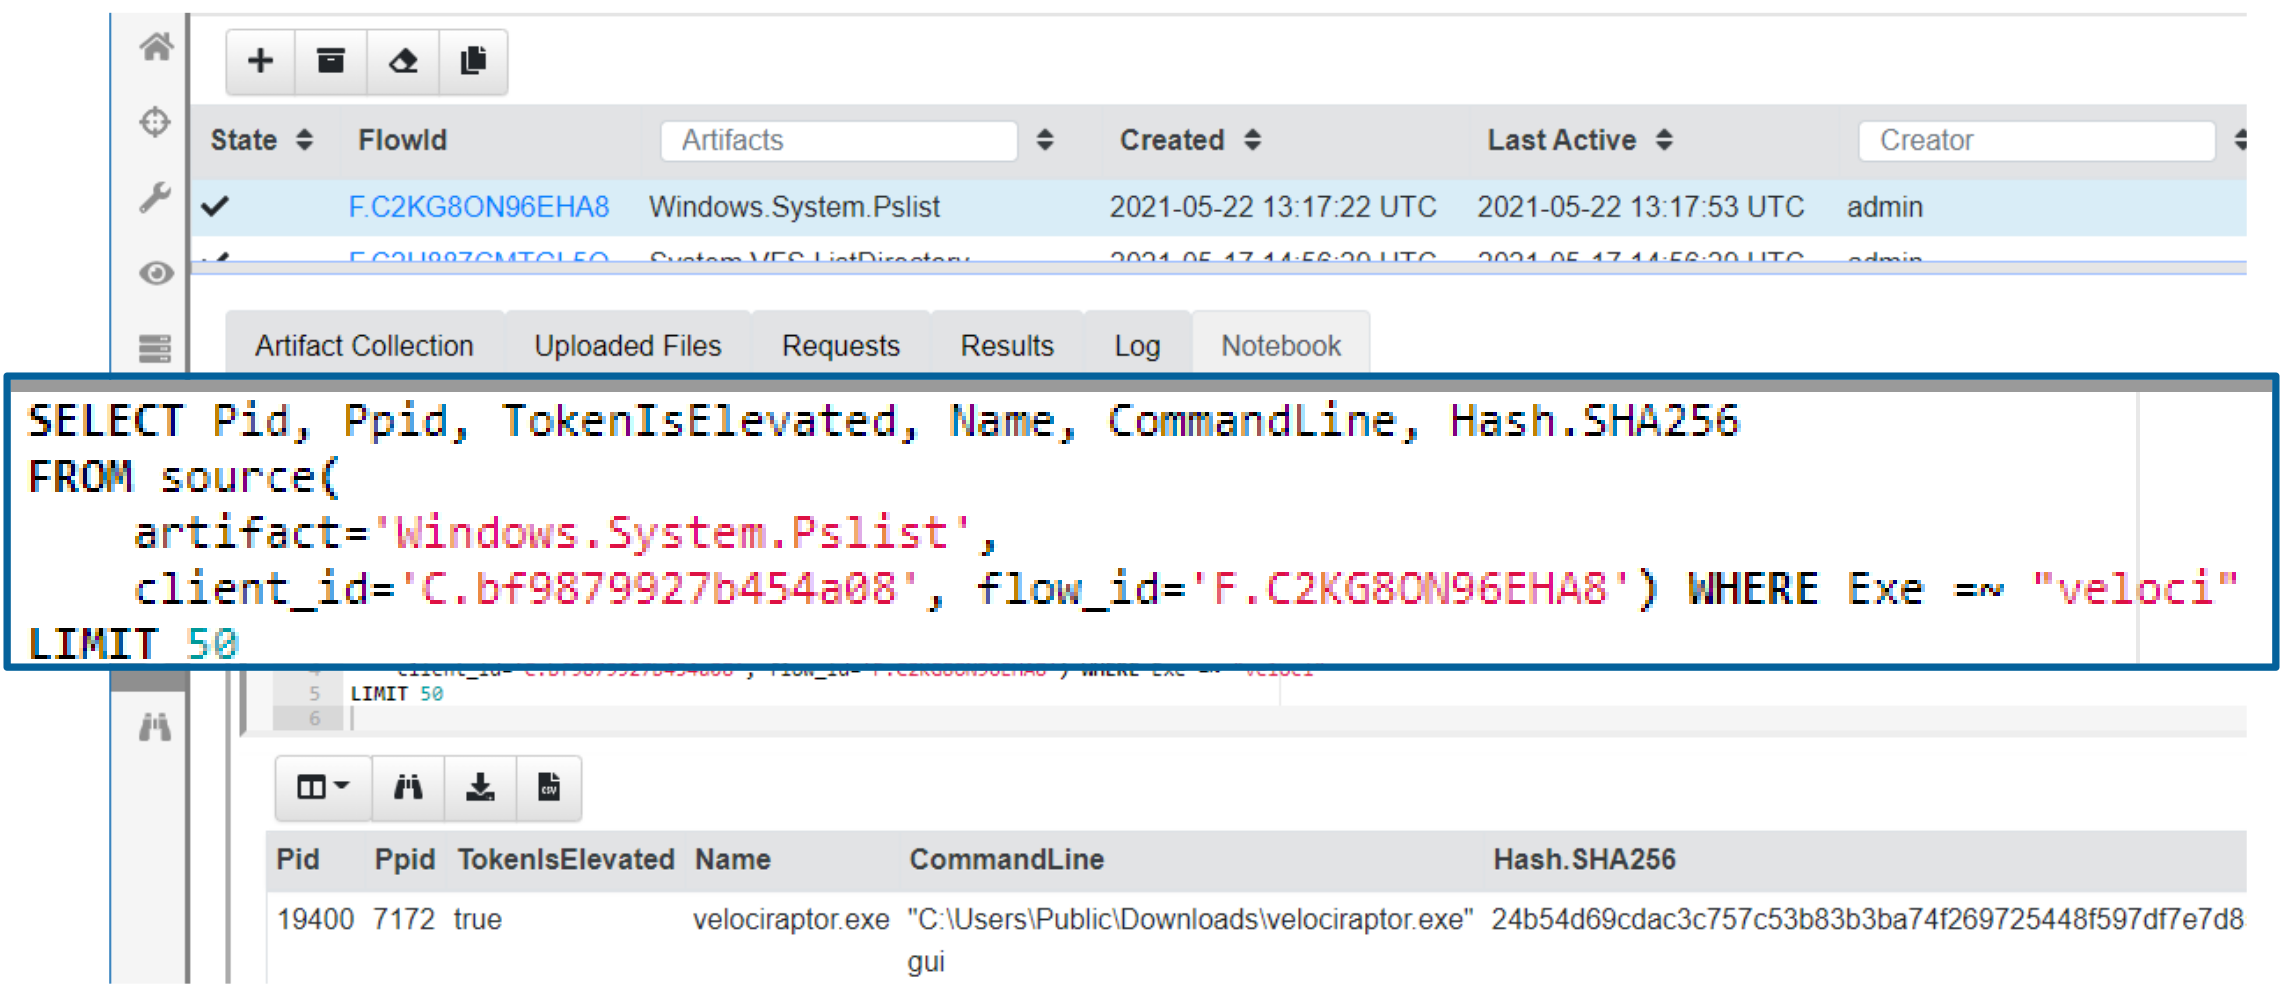
\includegraphics[width=\textwidth]{resources/06-velociraptor-notebooks-5.png}
\end{itemize}

\subsection{Velociraptor Query Language}


\subsubsection*{Core Concepts}
\begin{itemize}
   \item SQL-like forensics query language
   \item Plugin-based architecture
   \item Real-time execution capability
\end{itemize}

\subsubsection*{Example Queries}
\begin{lstlisting}[basicstyle=\ttfamily]
# Process Enumeration
SELECT Name, CommandLine, Pid 
FROM pslist()

# File Search
SELECT FullPath, Size, ModifiedTime 
FROM glob(globs="C:/Users/**/*.exe")

# Network Monitoring
SELECT LocalAddress, RemoteAddress, State 
FROM netstat() 
WHERE State = "ESTABLISHED"

# Registry Analysis
SELECT FullPath, ValueData 
FROM read_reg_key(
   globs="HKEY_LOCAL_MACHINE/Software/Microsoft/Windows/CurrentVersion/Run/*"
)

# Memory Analysis
SELECT ProcessId, VAD.Start, VAD.End 
FROM winpmem()
WHERE ProcessId = 1234
\end{lstlisting}

\subsubsection*{Features}
\begin{itemize}
   \item Nested query support
   \item Aggregation functions
   \item Regular expressions
   \item Event monitoring
   \item Custom plugin integration
\end{itemize}

\subsubsection*{Basic Syntax}
\begin{lstlisting}[basicstyle=\ttfamily]
-- comment  // Alternate comment style

// String matching
SELECT * FROM pslist() WHERE Exe =~ "veloci"

// Variable assignment
LET test = "gugus"
LET test = SELECT * FROM pslist()   // Reference query
LET test <= SELECT * FROM pslist()  // Store result

// Limit results
SELECT * FROM glob(globs="C:/**") LIMIT 5
\end{lstlisting}

\subsubsection*{File and Registry Operations}
\begin{lstlisting}[basicstyle=\ttfamily]
// Debug logging
SELECT Null FROM pslist() WHERE log(message="yeah, hit line")

// File search with glob
SELECT Name FROM glob(globs="C:/Users/**/Downloads/*.ex?") LIMIT 5

// Registry query
SELECT FullPath, Name, Data.type, Data.value FROM 
  glob(globs="HKEY_USERS/*/Software/**/*", accessor="reg")
\end{lstlisting}

\subsubsection*{Glob Wildcards}
\begin{itemize}
    \item \texttt{?} - Single letter
    \item \texttt{*} - Part of string
    \item \texttt{**} - Recursive folder traversal
\end{itemize}

\textbf{Note:} Always use forward slashes (/) for paths across platforms.

\subsection{YARA in Velociraptor}
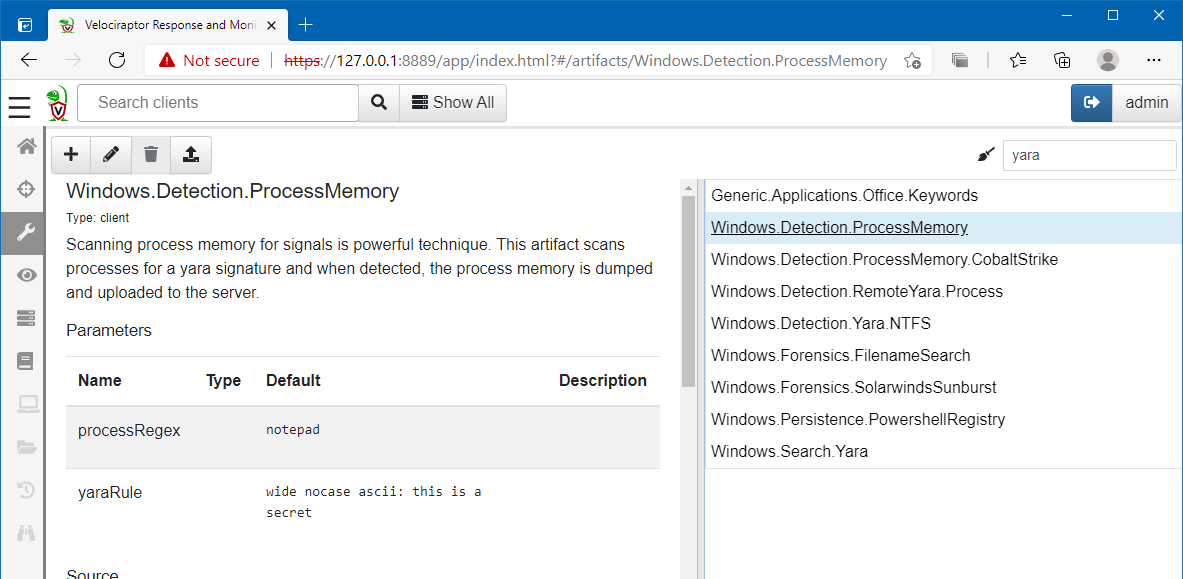
\includegraphics[width=\textwidth]{resources/06-yara.png}

Yara is a pattern matching tool used in Velociraptor for hunting malicious content. It allows creating rules to search for specific patterns in files and memory.

Key capabilities:
\begin{itemize}
  \item Define patterns using strings, hex, regular expressions
  \item Combine rules with boolean logic
  \item Match on file content, metadata, and process memory
  \item Integrate with Velociraptor's VQL for automated hunting
\end{itemize}

Example Yara rule in Velociraptor:

\begin{lstlisting}[basicstyle=\ttfamily]
- name: Detect_Suspicious_Script
  query: |
    SELECT * FROM Yara.Scan(
      files="C:\\Users\\*\\*.ps1",
      yara_rule='''
      rule Sus_PowerShell {
        strings:
          $s1 = "Invoke-Expression" nocase
          $s2 = "Net.WebClient" nocase
        condition:
          all of them
      }
      '''
    )
\end{lstlisting}

You can get yara rules from many sources (threat intel, blog posts etc)
YARA is really a first level triage tool:
\begin{itemize}
  \item Depending on signature many false positives expected
  \item Some signatures are extremely specific so make a great signal
\end{itemize}
Speed things up
\begin{itemize}
  \item Try to collect additional context around the hits to eliminate false positives.
\end{itemize}

Avoid DoS
\begin{itemize}
  \item Yara scanning is relatively expensive! Consider more targeted
\end{itemize}

\subsubsection*{Velociraptor YARA inline Hunt Example}

Let’s try to find something memory resident. Thus, you need to prepare a system with a specific string in memory.
Fire-up a Notepad* and enter some text. Well, it could be something else of course.

Try to find the “malicious” process and list its ID, name and executable path
\begin{itemize}
  \item Create a yara rule that hits the "specific string" or "some text" (string, and condition)
\end{itemize}

\begin{lstlisting}[basicstyle=\ttfamily]
LET r00l = 'rule detector { strings: $srch = "some text" condition : $srch }'
\end{lstlisting}

\begin{itemize}
  \item Enumerate all processes (pslist)
  \item For every process, do a yara\ search (proc\_yara, Pid)
\end{itemize}

\begin{lstlisting}[basicstyle=\ttfamily]
LET rule = 'rule dtect { strings: $srch = "Secret_Name" condition : $srch }'
LET pid = SELECT Pid, Exe, Name FROM pslist()
LET qry = SELECT Name, Exe, Pid from proc_yara( pid=Pid, rules=rule)
SELECT * FROM foreach(row=pid, query=qry)
\end{lstlisting}

\subsection{Logs}
\begin{lstlisting}[basicstyle=\ttfamily]
LET seclogs <= SELECT FullPath FROM
glob(globs="C:/Windows/System32/winevt/Logs/*Security*.evtx") LIMIT 3
SELECT *, timestamp(epoch=System.TimeCreated.SystemTime) as Time FROM
parse_evtx(filename=seclogs, accessor="ntfs") WHERE System.EventID.Value = 4624
ORDER BY Time
\end{lstlisting}

\subsubsection*{Conversion Example, Little Endian $\Rightarrow$ Big Endian}
\begin{lstlisting}[basicstyle=\ttfamily]
using System;
using System.Text;
namespace LEBEconversion
{
  class Program
  {
    static void Main(string[] args)
    {
      var source = "sumtin";
      var bytes = Encoding.BigEndianUnicode.GetBytes(source);
      var result = Encoding.Unicode.GetString(bytes);
      Console.WriteLine(result);
    }
  }
}
\end{lstlisting}

\subsubsection*{Dead Disk Forensics}
\begin{lstlisting}[basicstyle=\ttfamily]
// mount vmdk -> creates /mnt/flat
$ vmware-mount -f win10.vmdk /mnt
// auto generate mapping file
// alternatively use disk.dd instead of /mnt/flat
$ velo-linux-amd64 -v deaddisk --add_windows_disk /mnt/flat remapping.yaml
// let us have a look
$ velo-linux-amd64 --config_override remapping.yaml gui -v
\end{lstlisting}

\section{exercise}
